%versi 3 (22-07-2020)
\chapter{Landasan Teori}
\label{chap:teori}

\section{KIRI}
\label{sec:kiri}
KIRI (lihat Gambar \ref{fig:tampilanawalkiri}) adalah sebuah situs web navigasi transportasi umum berbasis web yang menyediakan rute antara dua lokasi geografis menggunakan transportasi publik. KIRI dirancang untuk melayani kebutuhan pengguna angkot (angkutan kota) di Bandung serta TransJakarta dan Commuterline di DKI Jakarta. Salah satu keunggulan KIRI dibandingkan layanan seperti Google Maps atau Moovit adalah kemampuannya memahami karakteristik  transportasi publik, di mana penumpang dapat naik atau turun di sepanjang jalan tanpa terbatas pada halte tertentu.
\begin{figure}[H] 
	\centering  
	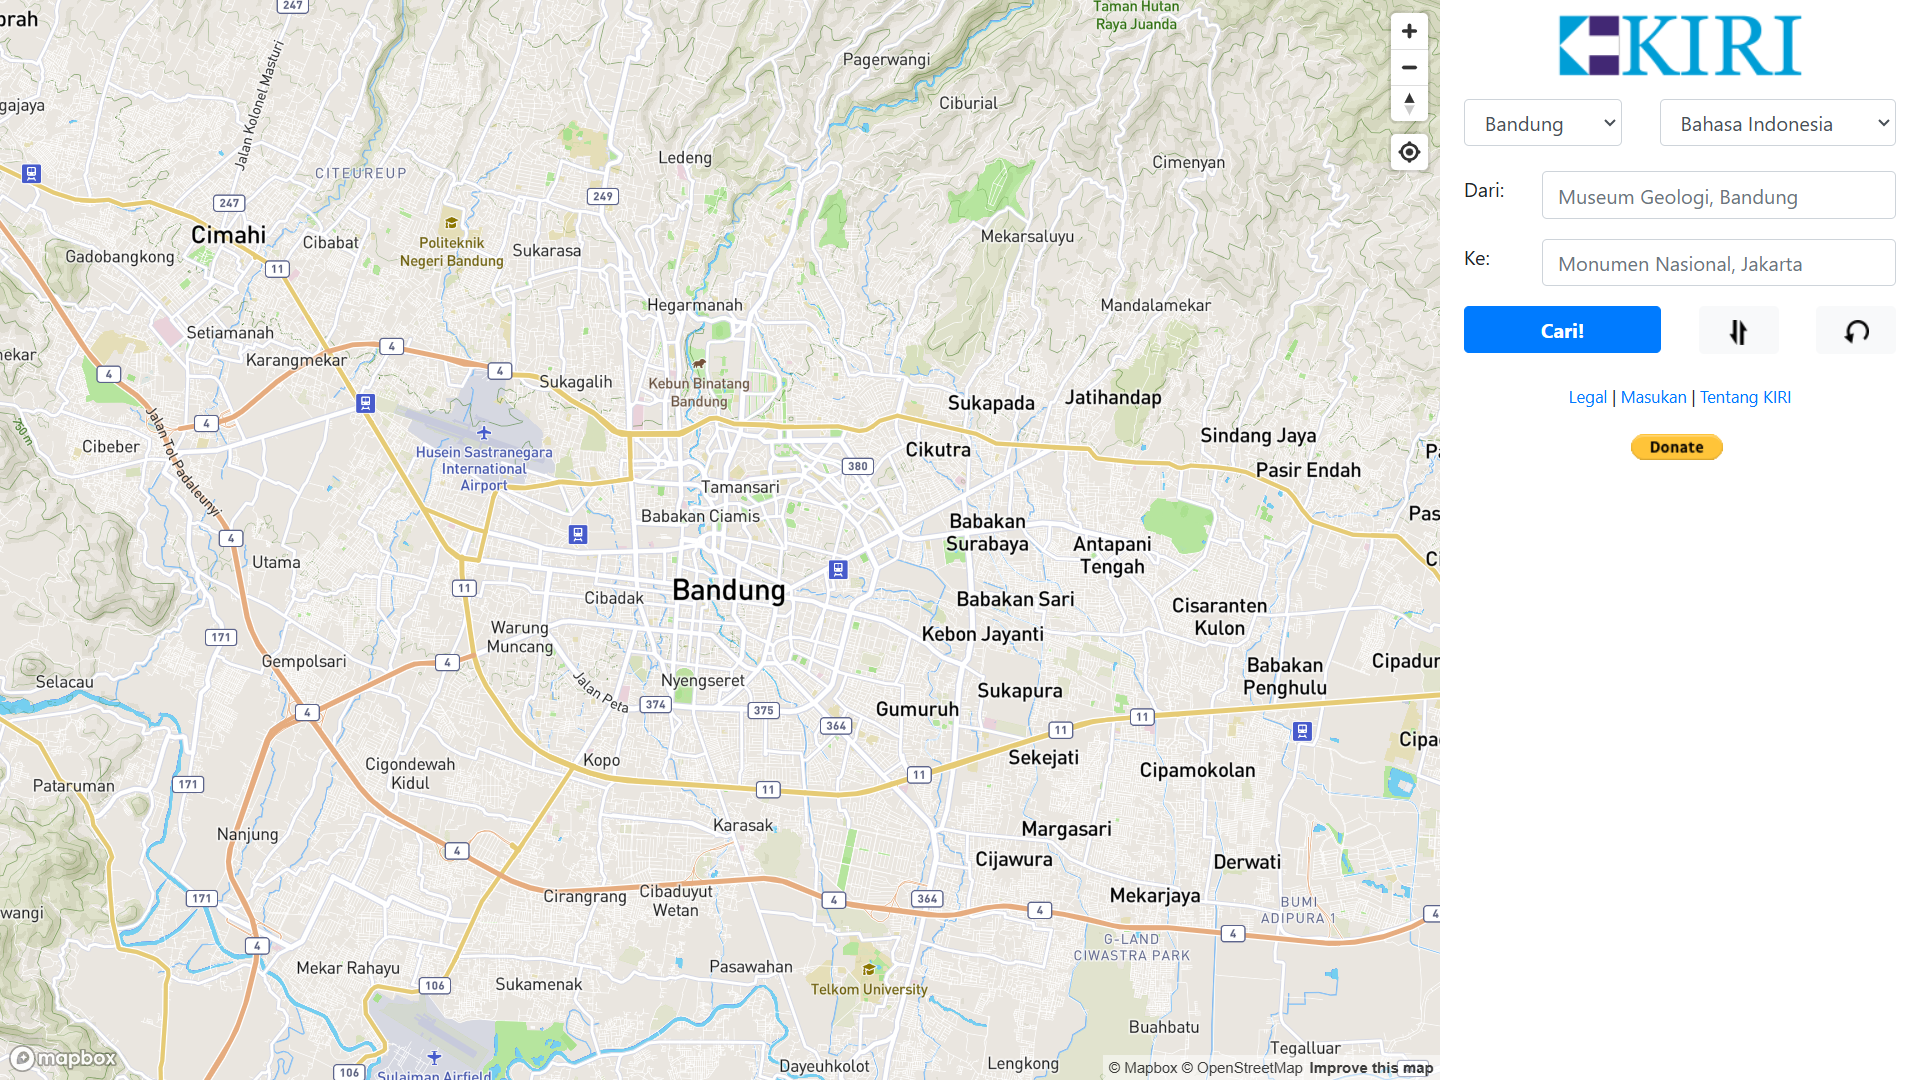
\includegraphics[width=1\textwidth]{KIRI}  
	\caption{Tampilan awal perangkat lunak KIRI}
	\label{fig:tampilanawalkiri} 
\end{figure}
\newpage
\noindent
KIRI akan memberikan informasi mengenai langkah-langkah yang harus ditempuh oleh pengguna yang akan berpergian dari satu tempat ke tempat tujuannya, mulai dari seberapa jauh pengguna harus berjalan untuk menaiki angkot yang bersangkutan, di mana pengguna harus naik atau turun angkot tersebut, seberapa jauh lagi pengguna harus berjalan sampai ke lokasi tujuan, dan seberapa lama estimasi waktu perjalanan yang akan ditempuh (lihat Gambar \ref{fig:tampilankiri}).
\begin{figure}[H] 
	\centering  
	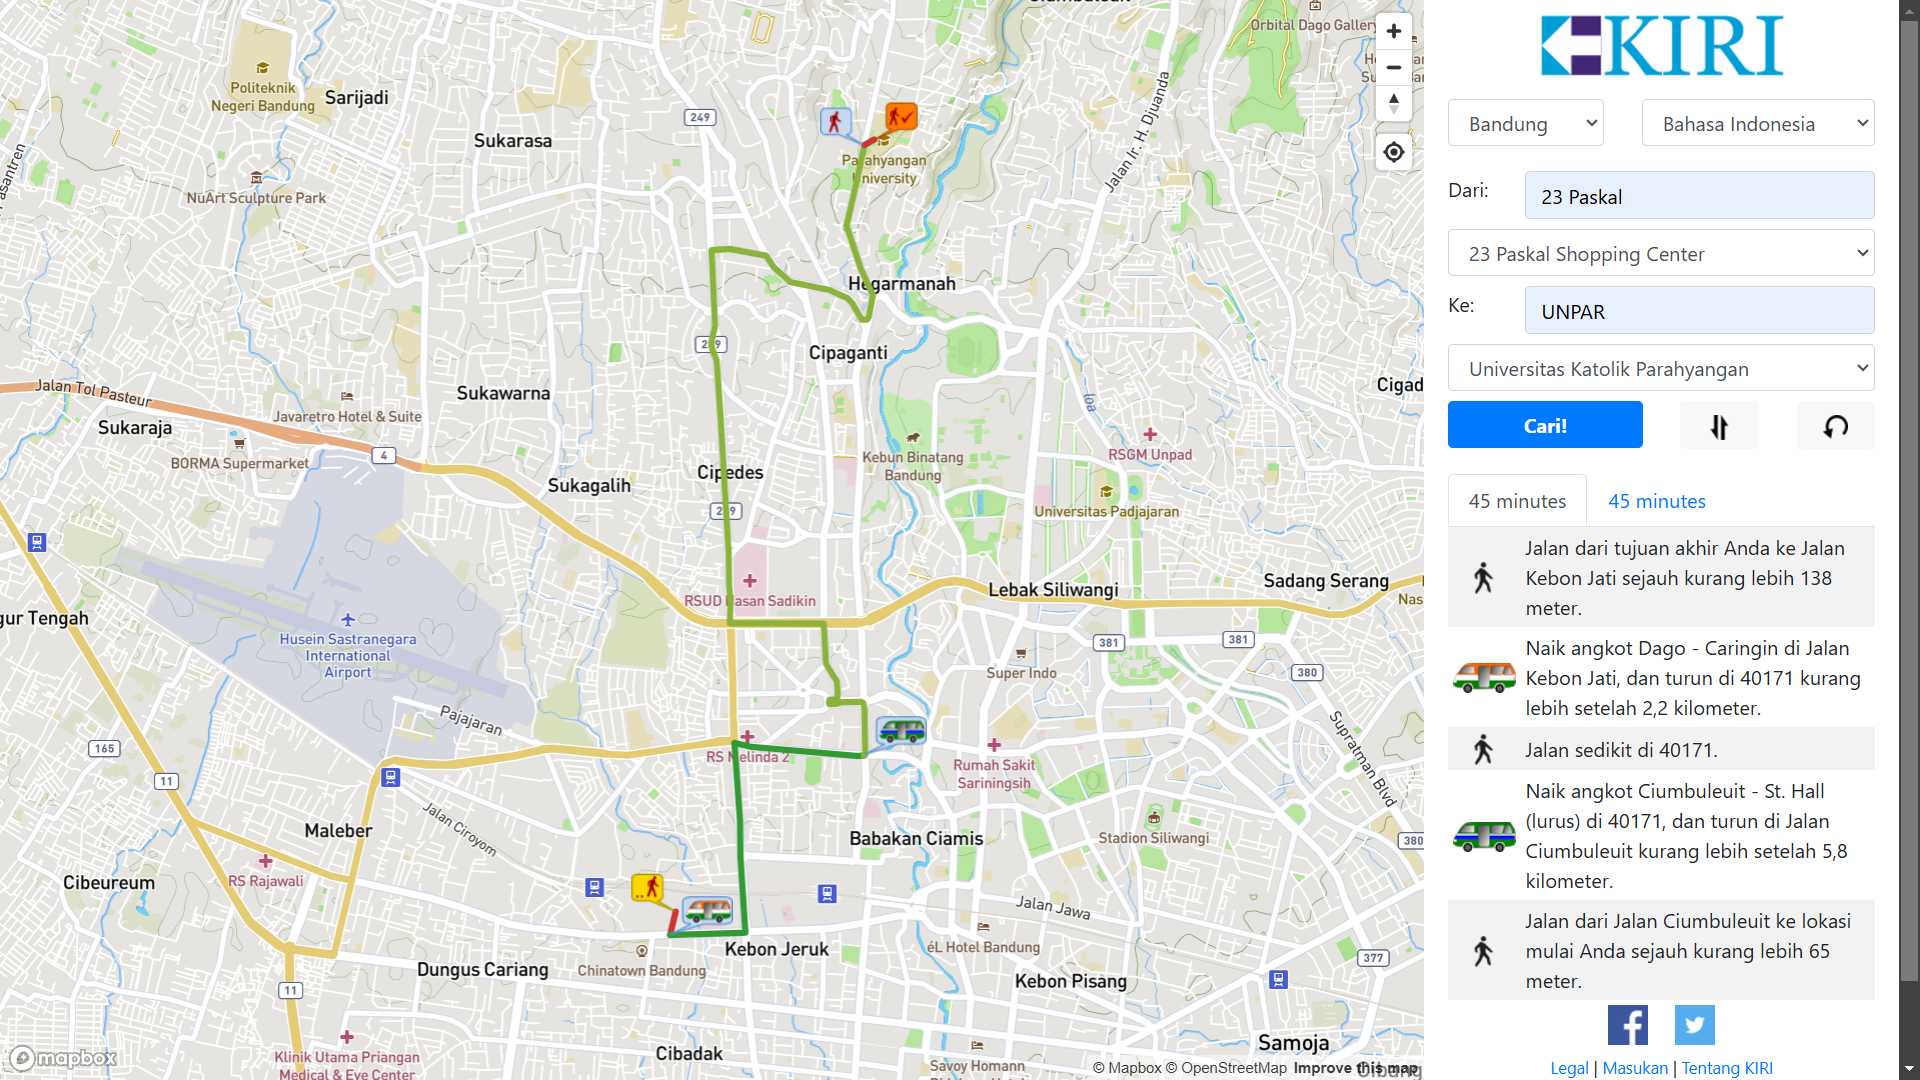
\includegraphics[width=1\textwidth]{KIRI-2}  
	\caption{Tampilan perangkat lunak KIRI, setelah menerima masukan}
	\label{fig:tampilankiri} 
\end{figure}
\noindent
Arsitektur aplikasi KIRI terbagi menjadi dua bagian utama. Yang pertama, yaitu Tirtayasa yang merupakan bagian \textit{frontend} dari KIRI, dan bertanggung jawab sebagai antarmuka pengguna untuk browser web. Komponen ini mengubah nama tempat yang dimasukkan pengguna menjadi koordinat geografis dengan menggunakan bantuan Google Maps. Tirtayasa sendiri dibangun menggunakan PHP dan Framework CodeIgniter 4.
\\
Selanjutnya, NewMenjangan, yang merupakan bagian \textit{backend} dari KIRI dan dibangun dengan bahasa pemrogrman Java serta digunakan untuk memproses permintaan navigasi. Komponen ini memuat semua jalur transportasi umum dalam bentuk graf dan menggunakan algoritma Dijkstra untuk menghitung rute optimal. Algoritma ini dipercepat dengan penggunaan struktur data heap, yang membuatnya efisien untuk jalur yang kompleks.

\section{Design Pattern dan Strategy Pattern}
\label{sec:designpattern}
~\cite{Gamma:94:design}
\textit{Design Pattern} adalah solusi umum yang telah terbukti efektif untuk mengatasi masalah desain berulang dalam pengembangan perangkat lunak berorientasi objek. Solusi ini dirancang agar dapat digunakan kembali di berbagai konteks tanpa harus disesuaikan secara berlebihan. Sebagai contoh, pola desain membantu memecah masalah desain menjadi struktur yang lebih modular dan fleksibel, sehingga mempermudah pengembangan dan pemeliharaan perangkat lunak.
\\
Pada dasarnya, \textit{design pattern} memiliki empat elemen utama. Pertama, nama pola yang memberikan cara singkat untuk menyebut masalah desain tertentu, solusinya, dan konsekuensi dari penerapannya. Kedua, masalah, yaitu deskripsi konteks atau situasi di mana pola desain ini relevan. Ketiga, solusi, berupa abstraksi dari elemen-elemen desain dan kolaborasinya tanpa menyebutkan implementasi konkret. Keempat, konsekuensi, yang mencakup hasil dari penerapan pola, termasuk dampak pada fleksibilitas, efisiensi, dan pengelolaan sistem.
\\
Penggunaan \textit{design pattern} juga memungkinkan sistem menjadi lebih adaptif terhadap perubahan kebutuhan. Pola seperti \textit{Strategy} mempermudah pergantian algoritma di runtime, sedangkan \textit{Factory Method} membantu mengurangi ketergantungan pada implementasi spesifik dengan menyediakan cara fleksibel untuk membuat objek. Dengan demikian, design pattern mempermudah kolaborasi dan komunikasi antar tim pengembang.
\\
\textit{Strategy Pattern} merupakan salah satu pola desain perilaku yang dirancang untuk mendefinisikan serangkaian algoritma, mengenkapsulasi setiap algoritma, dan memungkinkan algoritma-algoritma tersebut untuk saling dipertukarkan. Pola ini memungkinkan algoritma untuk bervariasi. Dengan demikian, pengguna tidak perlu mengetahui detail implementasi dari algoritma yang digunakan, melainkan cukup berinteraksi melalui antarmuka umum yang disediakan oleh objek strategi.
\\
Pola ini sangat berguna ketika terdapat kebutuhan untuk mendukung berbagai varian algoritma dalam menyelesaikan tugas yang sama. \textit{Strategy Pattern} memindahkan setiap algoritma ke dalam kelas terpisah, yang disebut sebagai \textit{ConcreteStrategy}. Klien dapat memilih dan menyuntikkan strategi yang sesuai ke dalam konteks pada waktu eksekusi, sehingga memberikan fleksibilitas yang tinggi dalam proses pengembangan perangkat lunak.
\\
Manfaat utama dari \textit{Strategy Pattern} adalah kemampuannya untuk menghilangkan kompleksitas yang diakibatkan oleh penggunaan pernyataan kondisional yang rumit dalam kode, serta kemudahan dalam menambahkan atau mengganti algoritma tanpa perlu memodifikasi kode klien atau konteks. Namun, penerapan pola ini juga memiliki kelemahan, seperti meningkatnya jumlah kelas dalam sistem dan potensi timbulnya overhead komunikasi antara konteks dan strategi. Oleh karena itu, penerapan \textit{Strategy Pattern} sebaiknya dipertimbangkan dengan cermat, terutama dalam situasi di mana variasi algoritma memang diperlukan untuk memenuhi kebutuhan sistem.

\begin{figure}[h] 
	\centering  
	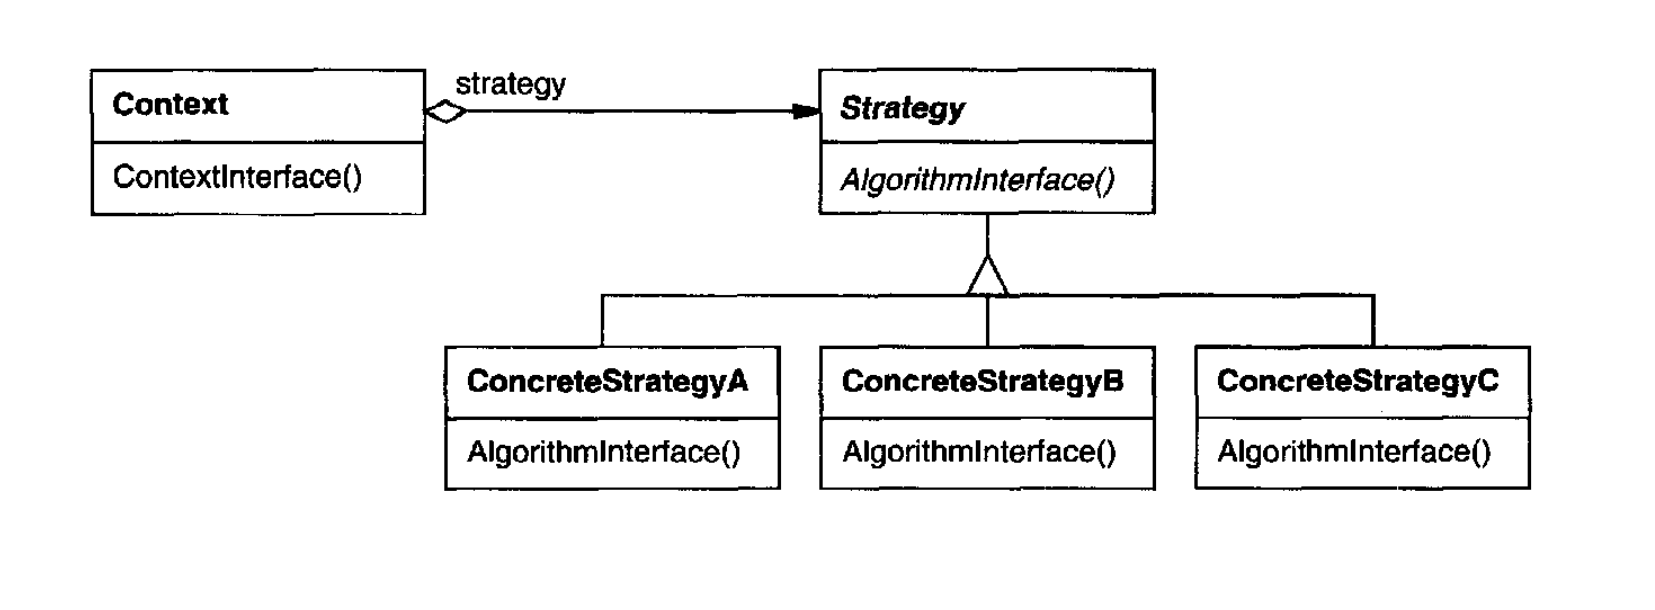
\includegraphics[width=1\textwidth]{struktur-sp}  
	\caption{Struktur Strategy Pattern}
	\label{fig:struktursp} 
\end{figure}

\subsection{Contoh Kode Program}
\label{sec:kode}


\section{MySQL}
\label{sec:mysql}
~\cite{oracle:24:mysql8.4}
MySQL merupakan sistem manajemen basis data relasional (\textit{Relational Database Management System}/RDBMS) bersifat open source yang dikembangkan oleh \textit{Oracle Corporation}. SQL, yang merupakan singkatan dari \textit{Structured Query Language}, adalah bahasa pemrograman yang digunakan untuk mengambil, memperbarui, menghapus, serta memanipulasi data pada basis data relasional.
\\
Sebagai basis data relasional, MySQL menyimpan data dalam bentuk tabel yang terdiri atas baris dan kolom, yang disusun dalam suatu skema. Skema ini bertugas mendefinisikan bagaimana data diorganisasi dan disimpan, serta menjelaskan hubungan antara tabel-tabel yang ada di dalamnya.
\\
Dalam MySQL, terdapat berbagai sintaks yang digunakan untuk mendukung pengelolaan basis data. Sintaks-sintaks tersebut mencakup operasi penting, seperti pembuatan tabel, penyisipan data, pembaruan data, penghapusan data, hingga pengambilan data. Setiap sintaks dirancang untuk mempermudah pengguna dalam mengelola data secara efektif dan efisien sesuai kebutuhan sistem. Berikut merupakan sintaks-sintaks dasar yang umum digunakan dalam MySQL.
\begin{itemize}
    \item \textbf{\textit{CREATE DATABASE}}
    \begin{lstlisting}[language=SQL]
    CREATE DATABASE database_name;
    \end{lstlisting}
    Sintaks tersebut digunakan untuk membuat database baru dalam MySQL. \texttt{database\_name} diisi nama dari database baru yang akan dibuat.
    \item \textbf{\textit{DROP DATABASE}}
    \begin{lstlisting}[language=SQL]
    DROP DATABASE database_name;
    \end{lstlisting}
    Sintaks tersebut digunakan untuk menghapus database yang telah dibuat dalam MySQL. \texttt{database\_name} diisi nama dari database yang akan dihapus.
    
    \item \textbf{\textit{CREATE TABLE}}
    \begin{lstlisting}[language=SQL]
    CREATE TABLE table_name (
        column1 datatype,
        column2 datatype,
        column3 datatype,
        ....
    );
    \end{lstlisting}
    Sintaks tersebut digunakan untuk membuat atau memasukan tabel baru kedalam sebuah database. \texttt{table\_name} diisi nama dari tabel yang akan dibuat, \texttt{column} diisi dengan nama kolom didalam tabel yang akan dibuat, dan \texttt{datatype} diisi dengan tipe data dari kolom yang akan dibuat, seperti \texttt{varchar}, \texttt{integer}, \texttt{date}, dan lain-lain.

    \item \textbf{\textit{DROP TABLE}}
    \begin{lstlisting}[language=SQL]
    DROP TABLE table_name;;
    \end{lstlisting}
    Sintaks tersebut digunakan untuk menghapus tabel yang telah dibuat dalam sebuah database. \texttt{table\_name} diisi nama dari tabel yang akan dihapus.

    \item \textbf{\textit{SELECT}}
    \begin{lstlisting}[language=SQL]
    SELECT column1, column2, ...
    FROM table_name;
    \end{lstlisting}
    Sintaks tersebut digunakan untuk memilih atau mengambil data dari sebuah tabel dalam database. \texttt{column} diisi dengan nama kolom dari sebuah tabel yang datanya akan diambil dan \texttt{table\_name} diisi dengan nama tabel dimana kolom tersebut berada.

    \item \textbf{\textit{WHERE}}
    \begin{lstlisting}[language=SQL]
    SELECT column1, column2, ...
    FROM table_name
    WHERE condition;
    \end{lstlisting}
    Sintaks tersebut digunakan untuk memilih atau mengambil data dari sebuah tabel dalam database dengan sebuah kondisi tertentu yang bertujuan untuk memfilter data yang akan diambil. \texttt{column} diisi dengan nama kolom dari sebuah tabel yang datanya akan diambil, \texttt{table\_name} diisi dengan nama tabel dimana kolom tersebut berada, dan \texttt{condition} diisi dengan kondisi dari data yang akan diambil atau filter seperti apa yang dingin dilakukan ketika mengambil data.

    \item \textbf{\textit{INSERT INTO}}
    \begin{lstlisting}[language=SQL]
    INSERT INTO table_name (column1, column2, column3, ...)
    VALUES (value1, value2, value3, ...);
    \end{lstlisting}
    Sintaks tersebut digunakan untuk memasukan atau menambahkan data baru kedalam kolom dari sebuah tabel yang telah ada. \texttt{tabel\_name} diisi nama tabel yang akan ditambahkan data baru, \texttt{column} diisi dengan nama kolom yang akan ditambahkan data baru, dan \texttt{value} diisi dengan nilai atau value dari data baru yang akan ditambahkan.

    \item \textbf{\textit{DELETE}}
    \begin{lstlisting}[language=SQL]
    DELETE FROM table_name
    WHERE condition;
    \end{lstlisting}
     Sintaks tersebut digunakan untuk menghapus data baru kedalam kolom dari sebuah tabel yang telah ada. \texttt{tabel\_name} diisi nama tabel yang akan ditambahkan data baru, \texttt{column} diisi dengan nama kolom yang akan ditambahkan data baru, dan \texttt{value} diisi dengan nilai atau value dari data baru yang akan ditambahkan.
\end{itemize}

\subsection{LineString}
\label{subs:linestring}
~\cite{oracle:24:mysql8.4}
\textit{LineString} adalah tipe data geometris dalam MySQL yang mewakili jalur atau lintasan yang terdiri dari satu atau lebih segmen garis yang terhubung. Tipe data ini digunakan dalam Sistem Informasi Geografis (GIS) untuk merepresentasikan lintasan seperti jalan, sungai, atau rute perjalanan. Setiap \textit{LineString} terdiri dari urutan titik (point) yang memiliki koordinat (x, y) dan minimal memiliki dua titik untuk membentuk garis.
\\
Untuk memanipulasi dan menganalisis \textit{LineString}, MySQL menyediakan sejumlah fungsi bawaan. Sebelum fungsi tersebut digunakan, objek \textit{LineString} biasanya dikonversi ke bentuk geometris menggunakan fungsi ST\_GeomFromText(). Fungsi ini menerima teks representasi geometris, seperti $LineString(x1 y1, x2 y2, ...)$ dan mengubahnya menjadi objek geometris yang dapat diproses oleh fungsi GIS lainnya.
Berikut adalah beberapa fungsi penting yang dapat digunakan untuk bekerja dengan \textit{LineString}:
\begin{itemize}
    \item ST\_EndPoint(ls)
    \\ Mengembalikan titik akhir dari \textit{LineString} $ls$. Contoh:
    \begin{lstlisting}[language=SQL]
    SET @ls = 'LineString(1 1, 2 2, 3 3)';
    SELECT ST_AsText(ST_EndPoint(ST_GeomFromText(@ls))); 
    -- Hasil: 'POINT(3 3)'
    \end{lstlisting}
    
    \item ST\_IsClosed(ls)
    \\ Mengecek apakah \textit{LineString} $ls$ membentuk lintasan tertutup (titik awal dan akhir sama). Contoh: 
    \begin{lstlisting}[language=SQL]
    SET @ls = 'LineString(1 1, 2 2, 3 3, 1 1)';
    SELECT ST_IsClosed(ST_GeomFromText(@ls));
    -- Hasil: 1 (TRUE)
    \end{lstlisting}
    
    \item ST\_Length(ls)
    \\ Menghitung panjang total \textit{LineString} $ls$. Contoh: \begin{lstlisting}[language=SQL]
    SET @ls = 'LineString(1 1, 2 2, 3 3)';
    SELECT ST_Length(ST_GeomFromText(@ls));
    -- Hasil: 2.828427
    \end{lstlisting}

    \item ST\_NumPoints(ls)
    \\ Mengembalikan jumlah titik yang membentuk \textit{LineString} $ls$. Contoh: 
    \begin{lstlisting}[language=SQL]
    SET @ls = 'LineString(1 1, 2 2, 3 3)';
    SELECT ST_NumPoints(ST_GeomFromText(@ls));
    -- Hasil: 3
    \end{lstlisting}
    
    \item ST\_Point(ls, N)
    \\ Mengembalikan titik ke-$N$ pada \textit{LineString} $ls$. Contoh: \begin{lstlisting}[language=SQL]
    SET @ls = 'LineString(1 1, 2 2, 3 3)';
    SELECT ST_AsText(ST_PointN(ST_GeomFromText(@ls), 2));
    -- Hasil: 'POINT(2 2)'
    \end{lstlisting}
    
    \item ST\_StartPoint(ls)
    \\ Mengembalikan titik awal dari \textit{LineString} $ls$. Contoh: \begin{lstlisting}[language=SQL]
    SET @ls = 'LineString(1 1, 2 2, 3 3)';
    SELECT ST_AsText(ST_StartPoint(ST_GeomFromText(@ls)));
    -- Hasil: 'POINT(1 1)'
    \end{lstlisting}

\end{itemize}

\section{Graf}
\label{sec:graph}
~\cite{Diestel:17:graph}
Graf adalah struktur yang terdiri dari simpul (\textit{vertex}) dan sisi (\textit{edge}), di mana sisi menghubungkan pasangan simpul. Sebuah graf direpresentasikan sebagai pasangan $G=(V,E)$, dengan $V$ sebagai himpunan simpul dan $E$ sebagai himpunan sisi. Sisi diwakili oleh pasangan simpul yang terhubung. Graf dapat bersifat terarah (sisi memiliki arah) atau tidak terarah (sisi tidak memiliki arah).
\\
Simpul-simpul dalam graf dapat memiliki derajat tertentu, yaitu jumlah sisi yang menghubunginya. Sebuah graf disebut terhubung jika terdapat jalur antara setiap pasangan simpul. Jalur ini adalah urutan simpul yang dihubungkan oleh sisi. Selain itu, siklus adalah jalur tertutup di mana simpul awal dan akhir adalah sama. Teori graf juga mencakup konsep seperti pohon (graf terhubung tanpa siklus), graf bipartit (simpul dibagi menjadi dua himpunan yang saling bebas sisi), dan subgraf (bagian dari graf yang tetap mempertahankan struktur graf).
\\
Graf digunakan dalam berbagai hal, seperti jaringan komputer, rute transportasi, dan analisis hubungan sosial. Teori graf menyediakan dasar matematis untuk mempelajari struktur ini dan memberikan cara untuk memodelkan dan menyelesaikan masalah kompleks di berbagai bidang.

\section{Algoritma Shortest Path}
\label{sec:algoritmasp}
Ada berbagai jenis algoritma \textit{shortest path} yang dirancang untuk menemukan lintasan terpendek antara dua titik dalam sebuah graf. Algoritma ini memainkan peran penting dalam berbagai aplikasi, seperti sistem navigasi, perencanaan jaringan, analisis data geografis, dan pemecahan masalah rute optimal.
\\
Setiap algoritma memiliki pendekatan, kelebihan, dan keterbatasan masing-masing, yang menjadikannya lebih sesuai untuk situasi tertentu. Sebagai contoh, algoritma seperti \textit{Dijkstra} sangat cocok untuk graf dengan bobot positif, sementara \textit{Floyd-Warshall} lebih sesuai untuk menemukan lintasan terpendek pada semua pasangan titik dalam graf kecil. Di sisi lain, algoritma \textit{A*} dirancang khusus untuk mempercepat pencarian lintasan dengan memanfaatkan heuristik. Berikut pembahasan secara detail tiga algoritma \textit{shortest path} yang digunakan, yaitu \textit{Dijkstra}, \textit{Floyd-Warshall}, dan \textit{A*}.

\subsection{Algoritma Dijkstra}
\label{sec:dijkstra}
~\cite{Cormen:09:intro}
Algoritma Dijkstra merupakan sebuah algoritma untuk menyelesaikan masalah \textit{single-source shortest path}, yaitu menemukan jalur terpendek dari satu titik asal ke semua titik lainnya dalam sebuah graf berarah dengan bobot tepi non-negatif. Proses ini dimulai dengan menginisialisasi perkiraan jarak terpendek dari titik asal $s$ ke semua titik lain. Algoritma ini menggunakan sebuah struktur \textit{min-priority queue} (antrean prioritas minimum) yang menyimpan titik-titik dengan prioritas sesuai dengan perkiraan jarak terpendek mereka dari titik asal.
\\
Selama eksekusi, algoritma Dijkstra akan secara bertahap memindahkan titik dengan estimasi jarak terpendek dari antrean ke dalam satu set $S$, yang menampung titik-titik dengan jarak terpendek yang sudah final. Untuk setiap titik $u$ yang baru dipindahkan ke dalam set $S$, algoritma akan memeriksa setiap tetangganya $v$ dan memperbarui perkiraan jarak terpendek ke $v$ jika melalui $u$ memberikan jarak yang lebih pendek. Proses ini dikenal sebagai “relaksasi” tepi, yaitu memperbarui perkiraan jarak dan menunjuk $u$ sebagai pendahulu $v$ bila ditemukan jalur yang lebih optimal.
\\
Proses algoritma berlanjut hingga semua titik di graf telah diproses, sehingga jarak terpendek dari titik asal $s$ ke setiap titik yang dapat dijangkau sudah final. Kompleksitas waktu dari algoritma ini bergantung pada implementasi antrean prioritas yang digunakan, dengan menggunakan \textit{Fibonacci heap}, algoritma Dijkstra dapat mencapai kompleksitas $O(VlogV+E)$, yang efisien untuk graf yang jarang (sparse). Algoritma ini sangat bermanfaat dalam berbagai aplikasi yang melibatkan pencarian jalur terpendek, seperti sistem navigasi dan perutean jaringan.

\subsection{Algoritma Floyd-Warshall}
\label{floydwarshall}
~\cite{Cormen:09:intro}
Algoritma Floyd-Warshall merupakan sebuah algoritma untuk menyelesaikan masalah jalur terpendek untuk semua pasangan titik dalam graf berarah dengan menggunakan pendekatan pemrograman dinamis. Algoritma ini sangat berguna untuk graf yang memiliki bobot sisi negatif, selama tidak terdapat siklus dengan bobot negatif dalam graf tersebut. Pendekatan ini menghitung jalur terpendek antara semua pasangan titik dengan menggunakan tabel bobot antar titik dan mengulanginya secara bertahap untuk mencapai solusi optimal.
\\
Langkah pertama dalam algoritma ini adalah mempersiapkan matriks bobot jalur terpendek yang akan terus diperbarui. Algoritma memulai dengan menganggap setiap titik memiliki jalur langsung ke dirinya sendiri dengan bobot nol, sementara bobot antar titik lain mengikuti nilai bobot sisi pada graf. Secara rekursif, algoritma memperbarui jalur terpendek dengan menambahkan titik perantara secara bertahap, yaitu jika titik $k$ menjadi perantara dari titik $i$ ke $j$, maka bobot jalur terpendek $d_{ij}$ akan diperbarui menjadi minimum dari $d_{ij}$ atau $d_{ik} + d_{kj}$. Proses ini mengoptimalkan semua jalur antara pasangan titik dengan menambahkan satu titik perantara setiap kali iterasi dilakukan.
\\
Algoritma Floyd-Warshall memiliki kompleksitas waktu $O(V^3)$ karena terdiri dari tiga lapisan perulangan untuk semua titik dalam graf, dengan V sebagai jumlah titik. Meskipun kompleksitasnya tinggi, algoritma ini cukup praktis untuk graf ukuran sedang dan memiliki struktur yang sederhana sehingga dapat diimplementasikan secara efisien. Selain itu, hasil algoritma ini dapat digunakan untuk mendeteksi siklus dengan bobot negatif dalam graf, jika ada nilai negatif pada diagonal utama dari matriks akhir, maka graf tersebut memiliki siklus negatif.
\\
Algoritma ini juga memungkinkan pencarian jalur terpendek melalui matriks pendahulu yang mencatat titik sebelumnya pada jalur terpendek untuk setiap pasangan titik. Dengan matriks ini, jalur terpendek antara titik manapun dapat direkonstruksi secara efisien.

\subsection{Algoritma A*}
\label{a*}
~\cite{Russell:09:ai}
Algoritma A* adalah metode pencarian yang meminimalkan estimasi total biaya solusi dengan menggabungkan dua fungsi, yaitu  
$g(n)$ dan $h(n)$ Fungsi $g(n)$ menghitung biaya aktual dari titik awal hingga simpul $n$, sedangkan $h(n)$ memperkirakan biaya tersisa dari $n$ ke tujuan. Kombinasi ini menghasilkan $f(n) = g(n) + h(n)$, yang memberikan perkiraan total biaya solusi jika rute melalui simpul $n$. Algoritma ini biasanya dipilih karena dapat mencapai solusi yang optimal dan lengkap, terutama jika fungsi heuristik $h(n)$ memenuhi kriteria tertentu.
\\
Kondisi utama yang diperlukan agar algortima A* memberikan solusi optimal adalah heuristik $h(n)$ yang bersifat \textit{admissible}, yaitu tidak pernah melebih-lebihkan biaya ke tujuan, dan \textit{consistent} atau \textit{monotonic}, di mana nilai $h$ tidak menurun di sepanjang jalur. Dengan adanya heuristik yang memenuhi syarat ini, algoritma A* dapat menghindari eksplorasi simpul-simpul yang tidak relevan, mengurangi waktu dan memori yang dibutuhkan.
\\
Terdapat kendala utama dari algoritma A*, yaitu penggunaan memori yang besar karena algoritma ini perlu menyimpan semua simpul yang telah dihasilkan. Meskipun waktu komputasi dapat diatasi dengan baik, kebutuhan memori yang tinggi sering kali menjadi tantangan. Untuk mengatasi hal ini, terdapat varian A* seperti \textit{Iterative-Deepening A*} (IDA*) yang mengurangi kebutuhan memori tanpa mengorbankan optimalitas solusi, dengan biaya eksekusi yang sedikit lebih tinggi.